\chapter{The Histogram of Gradient Orientations of Signal Plots}
\label{chapter:three}

This Chapter presents and introduce the EEG feature extraction procedure based on the Histogram of Gradient Orientations.  This method is based on an extension and modification of the SIFT~\cite{Lowe2004} Descriptor which is used in Computer Vision to extract and map local regions of an image.  At the same time, this Chapter fill in and end the previous Chapter, describing how to mine the information from the Plot and build a feature out of it.

\section{Introduction}

%sinuplot, spectrogram, scalogram

The work of Edelman, Intrator and Poggio~\cite{cogprints561} on how the visual cortex sense features was the inspiration to the use of the histogram of gradient orientations to decode local information from images.  SIFT is composed of two parts.  The first one is the keypoint location identification and the second part is the description of the patch using the Histogram of Gradient Orientations~\footnote{It should not to be confused with HOG~\cite{Dalal2005}, the Histogram Of Gradients which is another method from Computer Vision based on similar ideas.  Actually, the descriptor part of the SIFT Method has no specific name, but as it is based on building a histogram of gradient orientations, that is the reason why it is described here in that way. }.  The SIFT algorithm is biomimetically inspired in how the visual cortex detects shapes by analyzing orientations~\cite{cogprints561}.  The patch description is also based on the Theory of Receptive Fields and other similar ideas~\cite{Lindeberg2013}.

\section{Feature Extraction: Histogram of Gradient Orientations}
\label{SIFT}

Previous Chapter describes how to generate an image containing the plot of a signal.  On this generated image $I$, a keypoint $\gls{kp}$ is placed on a pixel $(x_{kp}, y_{kp})$ over the image plot and a window around the keypoint is considered. A local image patch of size $\gls{Sx} \times \gls{Sy}$ pixels is constructed by dividing the window in $16$ blocks of size $\gls{Deltas}$ each one,  where $\gls{St}$  and $\gls{Sv}$ are the scale of the local patch. It is arranged in a $4 \times 4$ grid and the pixel $\gls{kp}$ is the patch center. 

A local representation of the signal shape within the patch can be described by obtaining the gradient orientations on each of the $16$ blocks and creating a histogram of gradients.  This technique is the basis of Lowe's SIFT Descriptor method. In order to calculate the histogram, the interval $[0-360]$ of possible angles is divided in $8$ bins, each one at $45$ degrees.

 Hence, for each spacial bin $ i,j = \{0,1,2,3\} $, corresponding to the indexes of each block $B_{i,j}$,  the orientations are accumulated in a  $3$-dimensional histogram $h$ through the following equation: 
 

\begin{equation}
 h(\theta,i,j) = 3 s \sum_{\mathbf{p}} w_\mathrm{ang}(\angle J(\mathbf{p}) - \theta)\, w_{ij}\left(\frac{\mathbf{p} - \mathbf{kp}}{3 s}\right)\, |J(\mathbf{p})|
\label{eq:histogram}
\end{equation}

\noindent  where $\mathbf{p}$ is a pixel from within the patch,  $\theta$ is the angle bin with $ \theta \in \{0, 45, 90, 135, 180, 225, 270, 315\} $,  $ |J(\mathbf{p})| $ is the norm of the gradient vector in the pixel $\mathbf{p}$ and it is computed using finite differences and $\angle J(\mathbf{p}) $ is the angle of the gradient vector.  The scalar $ w_\mathrm{ang}(\cdot) $  and vector $ w_{ij}(\cdot) $ functions are linear interpolations used by~\cite{Lowe2004} and \cite{Vedaldi2010} to provide a weighting contribution to eight adjacent bins.  They are calculated as  

\begin{equation}
 w_{ij}(\mathbf{v}) = w( v_x - x_i ) w( v_y - y_i ) 
\label{eq:ij}
\end{equation}

\begin{equation}
 w_\mathrm{ang}(\alpha) = \sum_{k} w( \frac{8\alpha}{2\pi} + 8r)
\label{eq:wang}
\end{equation}

\noindent where $x_i$ and $y_i$ are the spatial bin centers located in $ x_i,y_i = \{-\frac{3}{2},-\frac{1}{2},\frac{1}{2},\frac{3}{2}\} $. The function parameter $\mathbf{v} = ( v_x, v_y ) $ is a vector variable and $\alpha$ a scalar variable.  On the other hand, $r$ is an integer that can vary freely which allows the argument $\alpha$ to be unconstrained in terms of its values in radians. The interpolating function $w(\cdot)$ is defined as:

\begin{equation}
 w(z) = \max(0,|z|-1).
\label{eq:weighting}
\end{equation}

These binning functions conform a trilinear interpolation that has a combined effect of sharing the contribution of each oriented gradient between their eight adjacent bins in a tridimensional cube in the histogram space, and zero everywhere else.

Lastly, the fixed value of $ 3 $ is a magnification factor which corresponds to the number of pixels per each block when $s = 1$.  As the patch has  $16$ blocks and  $8$ bin angles are considered, a feature called \textit{descriptor} of $128$ dimension is obtained. 
%It can be observed that the histogram is computed by multiplying by $ |J(\mathbf{p})| $, so the method considers both, the magnitude and the orientation of the gradient vector. 

Fig.~\ref{fig:sampledescriptor} shows an example of a patch and a scheme of the histogram computation. In (A) a plot of the signal and the patch centered around the keypoint is shown. In (B) the possible orientations on each patch are illustrated.  Only the upper-left four blocks are visible.  The first eight orientations of the first block, are labeled from $1$ to $8$ clockwise. The orientations of the second block $ B_{1,2} $ are labeled from $9$ to $16$.  This labeling continues left-to-right, up-down until the eight orientations for all the sixteen blocks are assigned. They form the corresponding $\mathbf{kp}$-descriptor of $128$ coordinates. Finally, in (C) an enlarged image plot is shown where the oriented gradient vector for each pixel can be seen.

\begin{figure}[h!]
\centering
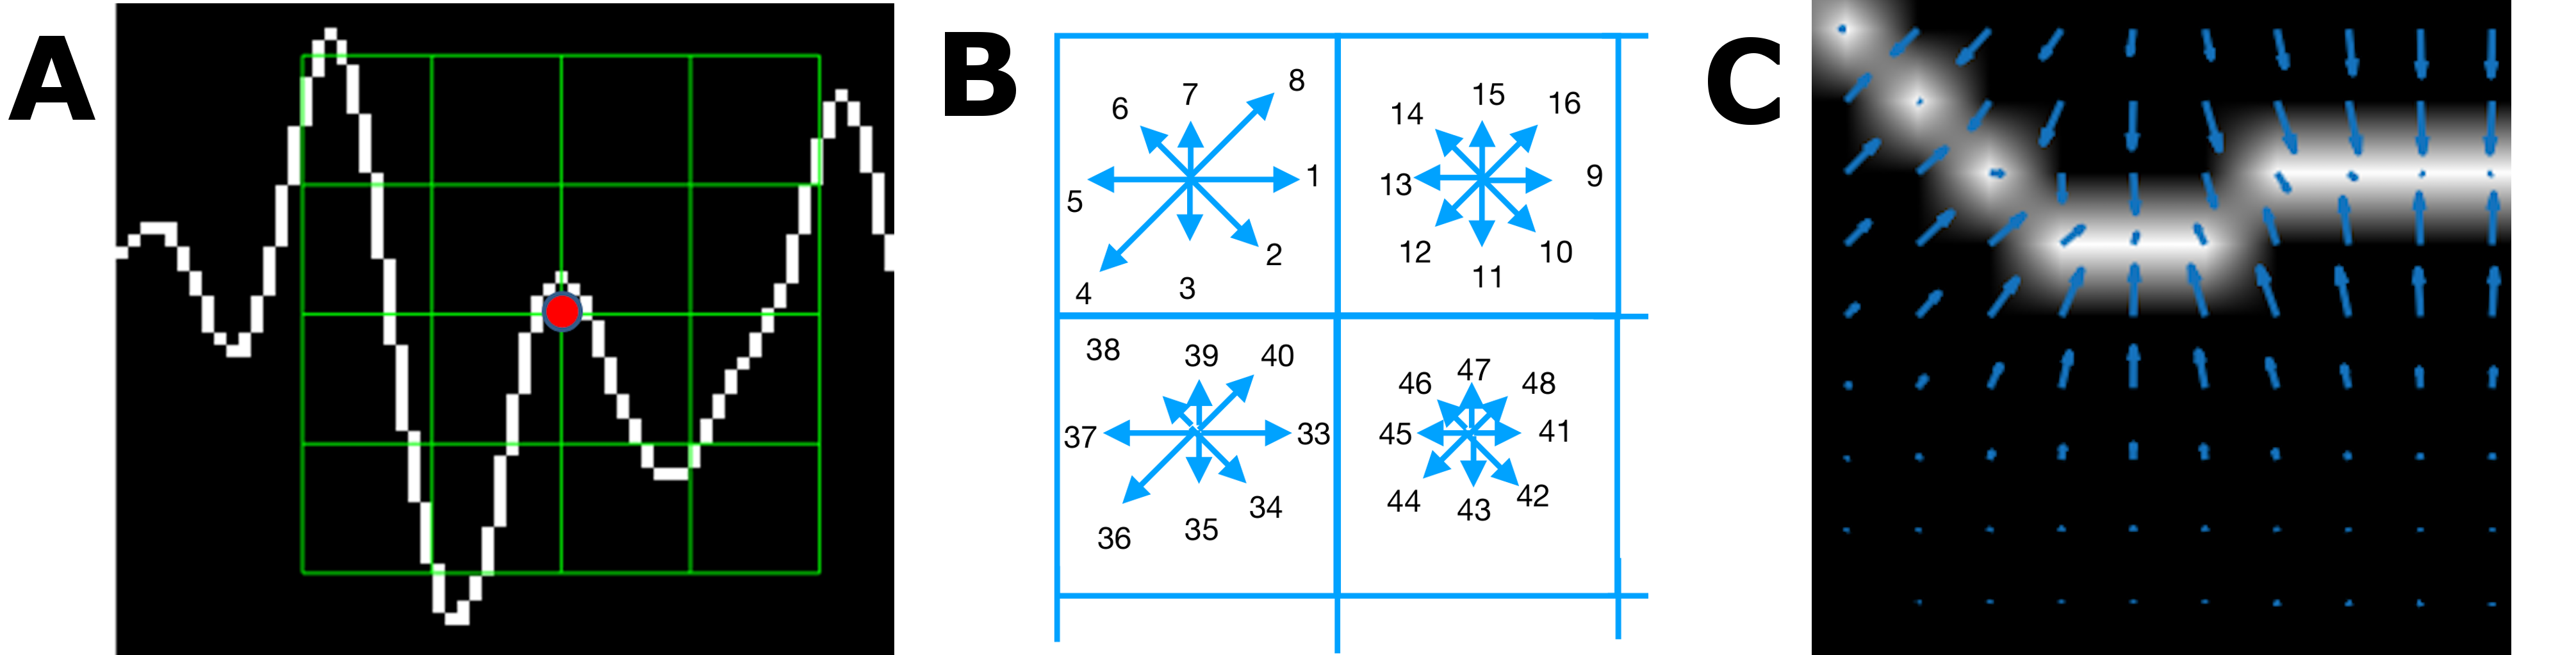
\includegraphics[width=16cm]{images/gradients.png}\label{samplegradients}
\caption[Histogram of Gradient Orientations for ERP]{ (A) Example of a plot of the signal, a keypoint and the corresponding patch. (B) A scheme of the orientation's histogram computation.  Only the upper-left four blocks are visible.  The first eight orientations of the first block, are labeled from $1$ to $8$ clockwise. The orientation of the second block $ B_{1,2} $ is labeled from $9$ to $16$.  This labeling continues left-to-right, up-down until the eight orientations for all the sixteen blocks are assigned. They form the corresponding descriptor of $128$ coordinates.  The length of each arrow represent the value of the histogram on each direction for each block. (C) Vector field of oriented gradients.  Each pixel is assigned an orientation and magnitude calculated  using finite differences. }
\label{fig:sampledescriptor}
\end{figure}

%\begin{figure}[h!]
%\centering
%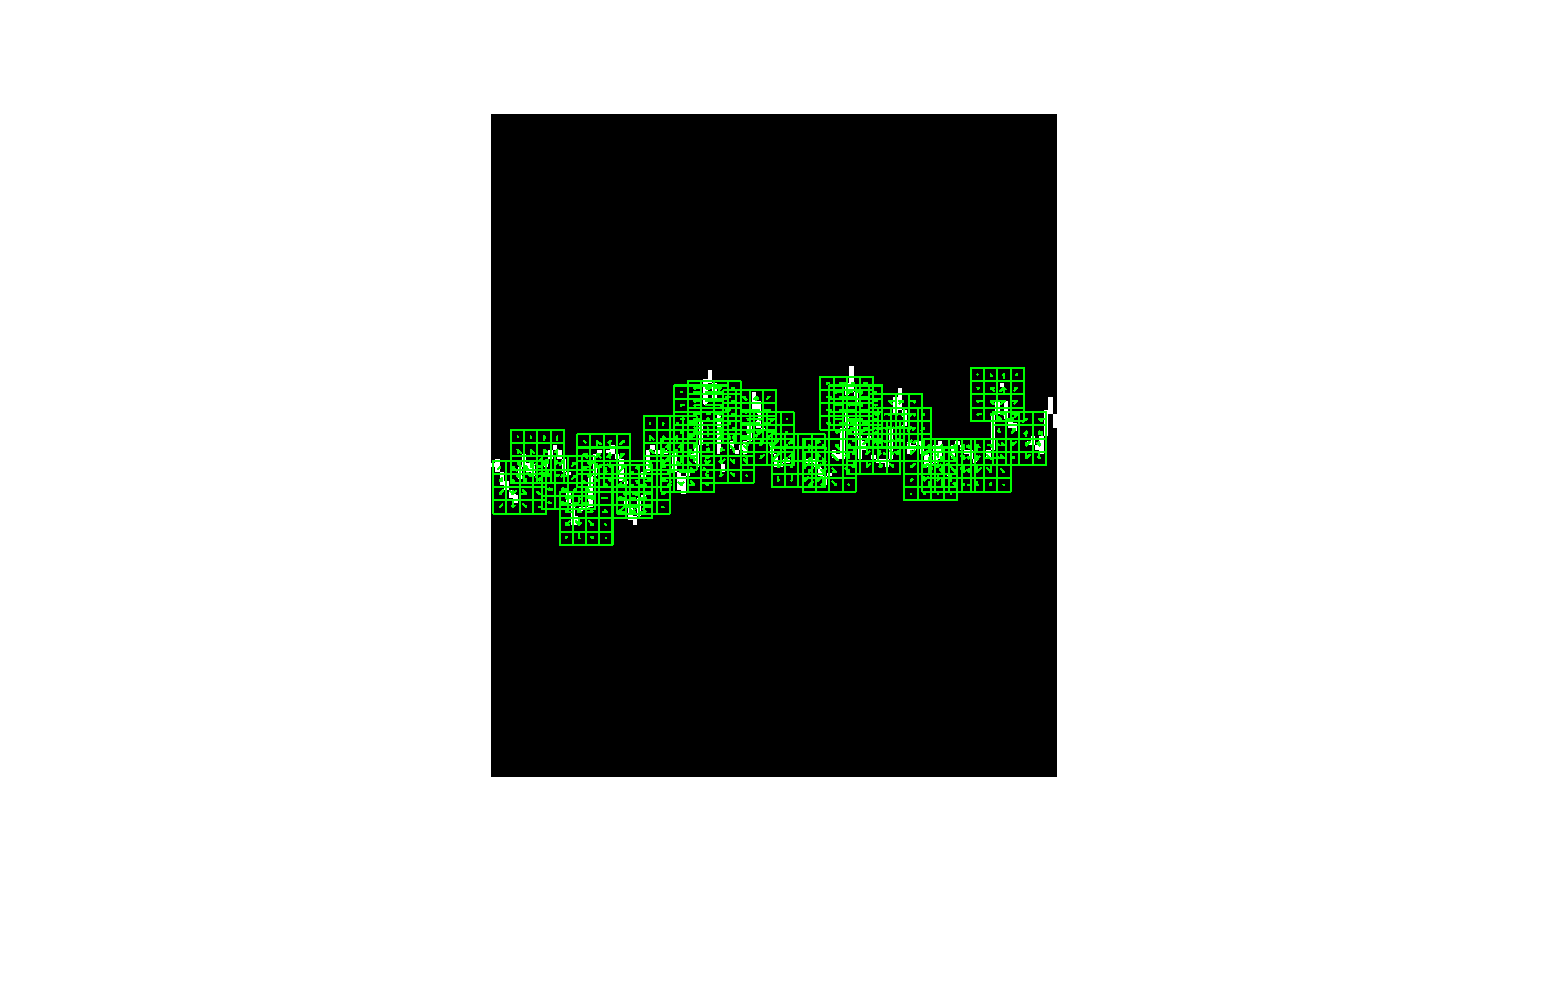
\includegraphics[scale=0.6]{images/KeypointLocations.eps}
%\caption[SIFT Patches]{fdsfdfsfs }
%\label{fig:siftpatch}
%\end{figure}

\section{Keypoint Location}

\begin{figure}[h!]
\centering
\subfigure[]
{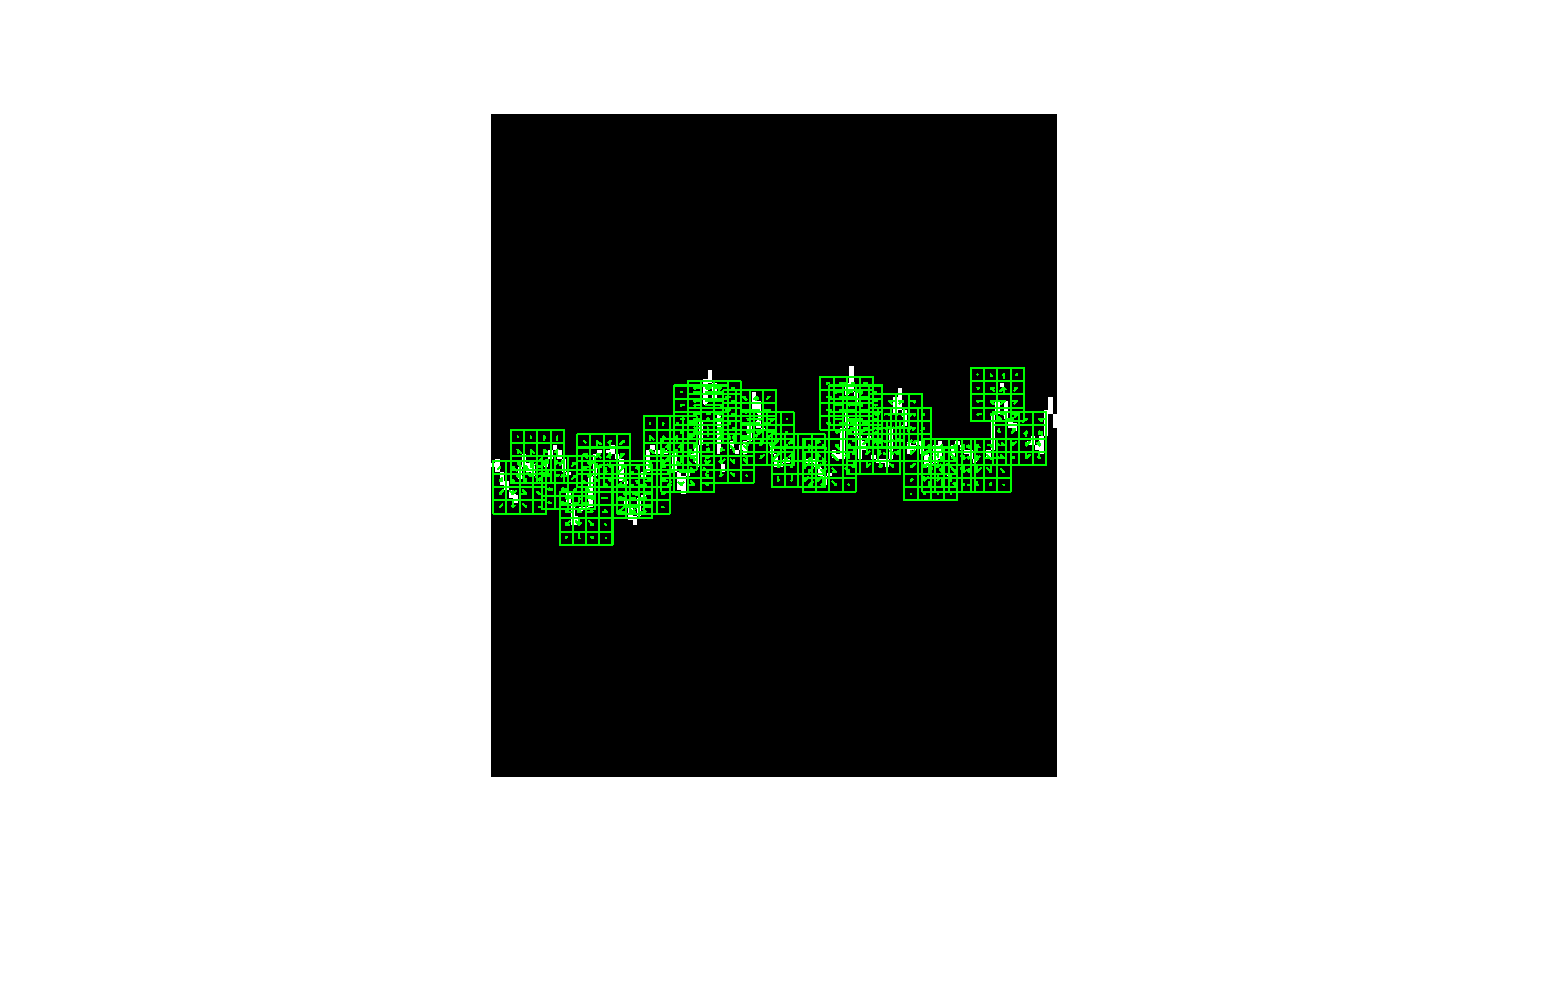
\includegraphics[width=6cm, height=6cm]{images/KeypointLocations.eps}}
\subfigure[]
{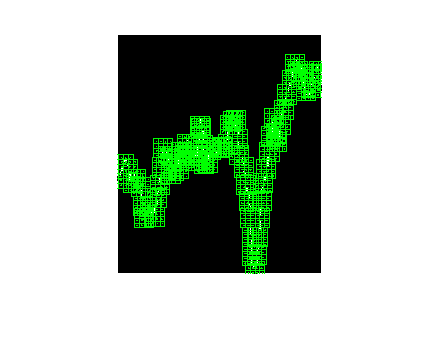
\includegraphics[width=6cm, height=6cm]{images/SignalWithFullDescriptors.png}}
\caption[Keypoint Locations]{}.
\label{fig:alpharesults}
\end{figure}

\subsection{Oscillatory Processes}

For these patterns, the central idea is to locate keypoints, and their patches and descriptors, all along the signal trace. 

\subsection{Transient Events}

For transient events, descriptors are treated as representatives of the signals itself so there is just one descriptor that is located in a meaningfull position along the time axis.

Additionally, particularly for autoscale plotting, the zero level can be used to localize keypoints.

\section{Mapping Functions}

This section contains a cheat-sheet with the mapping that allows to convert an EEG signal into an image and how the parameters of both are related.

$\gls{N}$, 
$\gls{lambda}$
$\gls{Fs}$
$\gls{Deltas}$
$\gls{DeltamuV}$
$\gls{gamma}$
$\gls{gammat}$
$\gls{Hy}$
$\gls{Wx}$
$\gls{St}$
$\gls{Sv}$
$\gls{Sy}$
$\gls{Sx}$
$\gls{w}$
$\gls{kp}$
$\gls{P}$

The initial parameters are $N$,$F_s$ and $\lambda$.  The unit length of the patch is $\Delta_s = \sqrt{2} \; 15$.  The peak-to-peak amplitude of the waveform to study is $ \Delta \mu V $.

Amplitude scale factor

\begin{equation}
\gamma \equiv \frac{H_y}{\Delta \mu V}  
\label{eq:gammadefinition}
\end{equation}

Time scale factor

\begin{equation}
\gamma_t \equiv \frac{W_x}{F_s \; w}  
\label{eq:gammatdefinition}
\end{equation}

%\begin{equation}
%s_x = \frac{ \gamma \;  \lambda \  F_s}{12}
%\label{eq:mapping2}
%\end{equation}
%
%\begin{equation}
%s_y= \frac{\gamma \; \Delta \mu V}{12} 
%\label{eq:mapping1}
%\end{equation}

Restriction on the waveform time scale

\begin{equation}
\frac{W_x-1}{\sqrt{2} \; 15}  \geq S_t 
\label{eq:restriction1}
\end{equation}

Restriction on the waveform amplitude scale

\begin{equation}
\frac{H_y-1}{\sqrt{2} \; 15}  \geq S_v 
\label{eq:restriction2}
\end{equation}

Waveform time scale

\begin{equation}
S_t = \frac{ \lambda \;  \  F_s \ \gamma_t }{\Delta_s}
\label{eq:mapping2}
\end{equation}

Waveform amplitude scale

\begin{equation}
S_v= \frac{\Delta \mu V \ \gamma}{\Delta_s} 
\label{eq:mapping1}
\end{equation}

Time to sample point conversion

\begin{equation}
n = \left\lfloor F_s \ \Delta_t \right\rfloor \ \gamma_t
\label{eq:mapping1}
\end{equation}

Horizontal Patch scale

\begin{equation}
\mathbf{S}_x = \Delta_s \; S_t + 1
\label{eq:mapping2}
\end{equation}

Vertical Patch scale

\begin{equation}
\mathbf{S}_y = \Delta_s \; S_v + 1
\label{eq:mapping1}
\end{equation}

Span of a Patch

\begin{equation}
\Delta_t = \frac{S_t \ \Delta_s}{F_s \ \gamma_t} 
\label{eq:mapping1}
\end{equation}


\section{Implementation}

\subsection{Matlab, C++ and VLFeat}

The histogram was implemented in this way.  Software was produced and published here and there.


\section{Classification}

A discriminative~\cite{WolpawJonathanR2012} semi-supervised classification method based on Naive Bayes Nearest Neighbor~\cite{Boiman2008} was applied to classify EEG signals using the features provided by the calculated descriptors.
One problem that frequently arises when using local features is how to go back from the classification of those local characteristics to the image where those descriptors came from.
The NBNN technique overcomes this problem by comparing each image against a whole class which is characterized by the set of descriptors that are closest to each one of the descriptors of the query image. This algorithm is very easy to implement, and is based on (5).

The estimated class C of a query image is calculated as the class C that minimize the summation of the L2 distance between each descriptor di that belongs to the query image and its corresponding near neighbot NNc(di) descriptor for each class.

In brief, based on segmented signals from at least two labeled classes, a set of images is first generated.  For each image, desctipros are extracted during the training or calibration step of a BCI procedure and they are grouped in KD-tree~\cite{Lowe2004} structures for each one of the classes.

Hence, given a new unlabeled signal segment, an image plot is generated as well, and their descriptors extracted.  They are fed into Equation 5 in order to determine the class which minimizes the summation and thus provide the information bit to the BCI controller.  


In order to identify the selected letter, the template set $T^{bpc}$ is used as a database.  Thus, new descriptors are computed and they are compared against the descriptors belonging to the calibration template set $T^{bpc}$.

\begin{itemize}

\item \textbf{Step D:} Match to the calibration template $T^{bpc}$ by computing  

\begin{equation}
\hat{row} = \arg \min_{l \in \{1,\dots,6\}} \sum_{q \in N_T(\mathbf{d}^{(l,bpc)})}^{} {\left\lVert q -  \mathbf{d}^{(l,bpc)} \right\rVert}  ^{2}
\label{eq:multiclassificationrow}
\end{equation}

\noindent and

\begin{equation}
\hat{col} = \arg \min_{l \in \{7,\dots,12\}} \sum_{q \in N_T(\mathbf{d}^{(l,bpc)})}^{} {\left\lVert q -  \mathbf{d}^{(l,bpc)} \right\rVert} ^{2}
\label{eq:multiclassificationcol}
\end{equation}

\noindent where $N_T(\mathbf{d}^{(l,bpc)})$  is defined as $N_T(\mathbf{d}^{(l,bpc)}) = \{\mathbf{d} \in T^{bpc} / $  is the k-nearest neighbor of $ \mathbf{d}^{(l,bpc)} \}$ for the best performing channel.  This set is obtained by sorting all the elements in $T^{bpc}$ based on distances between them and $\mathbf{d}^{(l,bpc)}$, choosing the $k$ with smaller values, with $k$ a parameter of the algorithm.  This procedure is based on the k-NBNN  algorithm~\cite{Boiman2008}.

\end{itemize}
By computing the aforementioned equations, the letter of the matrix can be determined from the intersection of the row $ \hat{row} $ and column $ \hat{col} $. 
Figure~\ref{fig:classification} shows a scheme of this process. 

\begin{figure}[h!]
\centering
\subfigure[Two Dictionaries contain templates descriptors for two different classes. A set of query descriptors are extracted from a new image that needs to be categorized.]
{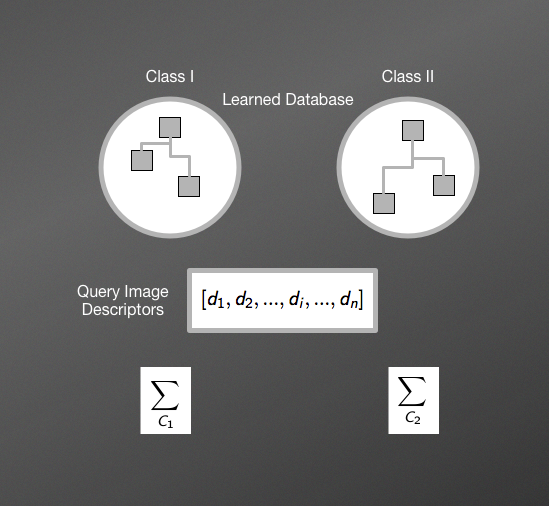
\includegraphics[height=6cm,width=4cm]{images/NBNNMethod1.png}}
\subfigure[Distances from every descriptor $di$ is calculated against the closest one from the Dictionary of Class 2.  Distances are accumulated. ]
{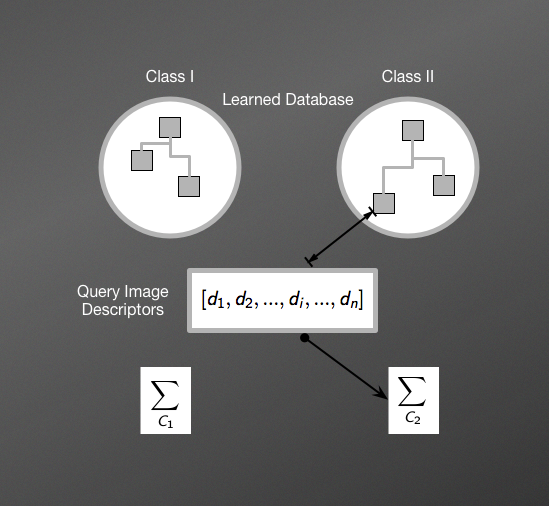
\includegraphics[height=6cm,width=4cm]{images/NBNNMethod2.png}}
\subfigure[Distances from every descriptor $di$ is calculated against the closest one from the Dictionary of Class 1.  Distances are accumulated. ]
{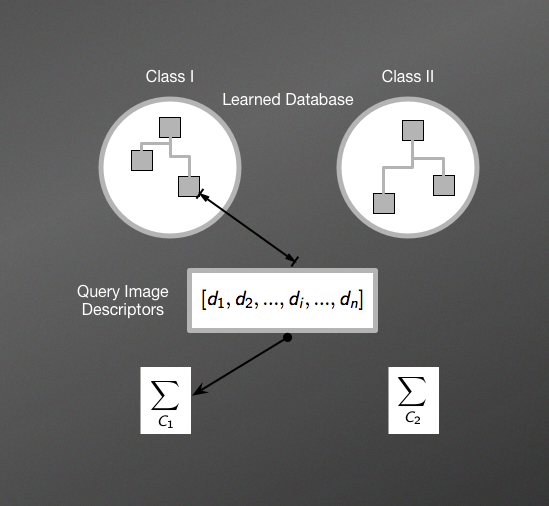
\includegraphics[height=6cm,width=4cm]{images/NBNNMethod3.png}}
\subfigure[The two different values are compared.]
{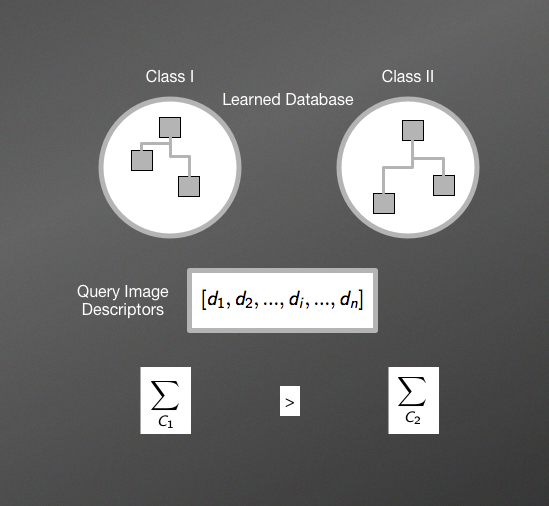
\includegraphics[height=6cm,width=4cm]{images/NBNNMethod4.png}}
\subfigure[The summation that achieved the lesser value is the one that more closely resemble the set of templates, thus is the one predicted by the classification algorithm. ]
{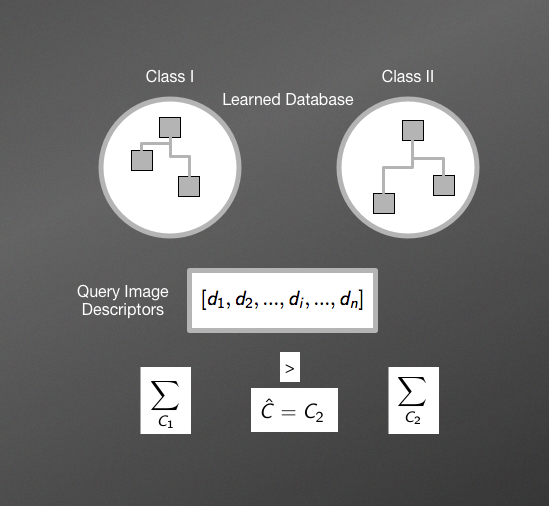
\includegraphics[height=6cm,width=4cm]{images/NBNNMethod5.png}}
\caption[NBNN Classification]{Classification Method.}
\label{fig:nbnnclassification}
\end{figure}



